\documentclass[times]{article}

\usepackage{graphicx}
\usepackage{placeins}
\usepackage[none]{hyphenat}
\usepackage{amsmath}
\usepackage[us]{datetime}
\usepackage[explicit]{titlesec}
\usepackage[margin=1.0in]{geometry}
\begin{document}
	\title{CS 6001 Applied Spatial and Temporal Data Analysis - Spring 2017 - Homework 2}
	\author{Dalton Cole}
	\date{\formatdate{27}{2}{2017}}
	\maketitle

	\section{Data Retrieval}
		\paragraph{}
		For this assignment, I had to retrive 100 CNN articles and convert them to a data matrix. This is done using the \textbf{scrapy.py} script, which is a python script. This script grabs the articles and title data from 100 CNN articles that have their URLs in \textbf{website\_list}. The articles must have at least 150 words to be considered a valid article. The articles used are in \textbf{used\_site\_list.txt}. For this experiment, all URLs in \textbf{website\_list} were used.

		\paragraph{}
		Five different categories of articles were used: Politics, Technology, Investment, Travel, and Health. These articles range over a wide time period but are about roughly the same subject (in respect to their categories).

		\paragraph{}
		The python script creates a data matrix with the article data. It counts the frequency of each word in each article and saves it in a csv file. The type of article is also stored in this file. The data is saved to \textbf{data.csv}�.
	
	\section{Classification}
		\paragraph{}
		Next, I had to run kNN and decision tree classifiers on the data matrix using 5-fold cross validation. The script used to run this is \textbf{kNN.py}. This file deals with both kNN and decision tree classification. The script takes the \textbf{data.csv} and sorts out the data into articles and article type. It then does kNN and decision tree classification on 5 different data sets, the 5-fold cross validation. The sklearn module in python was used for the kNN and decision tree classification.

		\subsection{kNN}
			\paragraph{}
			K-Nearest-Neighbors, or kNN for short, is a pattern matching algorithm used for classification. It works by looking at the k nearest neighbors after ``plotting'' the data. For example, in a two-dimensional grid, a new point would find the k nearest points. The point would then be classified as the same type as the majority of its neighbors. Essentially, the nodes around the point vote, whichever classification revives the most votes, wins. It is hard to visualize distance with over 11 thousand dimensions, but the basic concept still applies.

			\begin{figure}
				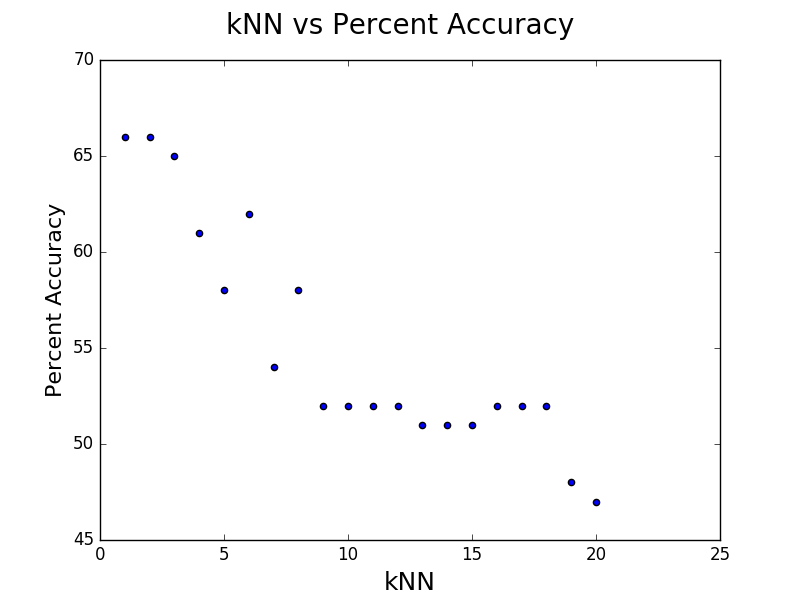
\includegraphics[width=\linewidth]{../kNNvsNum.png}
				\caption{kNN vs Percent Accuracy}
				\label{fig:kNNvsNum}
			\end{figure}

			\paragraph{}
			As can be seen by Figure \ref{fig:kNNvsNum}, one nearest neighbors had the highest accuracy at 69\%. Once it started looking at more neighbors, the accuracy gradually fell.

			\begin{table}[h!]
				\centering
				\resizebox{\textwidth}{!}{
				\begin{tabular}{ |c|c|c| } 
					 \hline
					 Nodes 	& Accuracy	& F-measure \\ 
					 \hline
					 1 		& 69.0\% 	& [0.65500000000000003, 0.67708333333333337, 0.53976190476190467, 0.57000000000000006, 0.79277777777777769] \\ 
					 2 		& 62.0\% 	& [0.65500000000000003, 0.56848739495798328, 0.57777777777777772, 0.49539682539682539, 0.57008547008547006] \\ 
					 3 		& 66.0\% 	& [0.65500000000000003, 0.67708333333333337, 0.51500000000000001, 0.44345238095238093, 0.75628815628815638] \\ 
					 4 		& 65.0\% 	& [0.65500000000000003, 0.62324929971988807, 0.51500000000000001, 0.44345238095238093, 0.74358974358974361] \\ 
					 5 		& 59.0\% 	& [0.55083333333333329, 0.52291666666666659, 0.40212121212121216, 0.46011904761904765, 0.64009740259740266] \\ 
					 6 		& 61.0\% 	& [0.65500000000000003, 0.52291666666666659, 0.40212121212121216, 0.47249999999999998, 0.64464285714285707] \\ 
					 7 		& 59.0\% 	& [0.65500000000000003, 0.53455882352941175, 0.33116883116883117, 0.42083333333333328, 0.64464285714285707] \\ 
					 8 		& 60.0\% 	& [0.65500000000000003, 0.53455882352941175, 0.33116883116883117, 0.47249999999999998, 0.64464285714285707] \\ 
					 9 		& 57.0\% 	& [0.60449494949494942, 0.56874999999999998, 0.23957219251336898, 0.47249999999999998, 0.56771978021978009] \\ 
					 10		& 56.0\% 	& [0.60449494949494942, 0.47622549019607846, 0.23957219251336898, 0.47249999999999998, 0.56771978021978009] \\ 
					 11		& 52.0\% 	& [0.60449494949494942, 0.356578947368421, 0.23957219251336898, 0.40666666666666662, 0.50593406593406598] \\ 
					 12		& 53.0\% 	& [0.65500000000000003, 0.356578947368421, 0.22857142857142859, 0.40666666666666662, 0.50593406593406598] \\ 
					 13		& 48.0\% 	& [0.49016483516483522, 0.18214285714285716, 0.23333333333333331, 0.40666666666666662, 0.50593406593406598] \\ 
					 14		& 48.0\% 	& [0.49016483516483522, 0.18214285714285716, 0.22974358974358972, 0.40428571428571425, 0.50593406593406598] \\ 
					 15		& 50.0\% 	& [0.49016483516483522, 0.33888888888888891, 0.22857142857142859, 0.40428571428571425, 0.50593406593406598] \\ 
					 16		& 49.0\% 	& [0.54162587412587415, 0.18214285714285716, 0.22974358974358972, 0.3997435897435897, 0.50593406593406598] \\ 
					 17		& 45.0\% 	& [0.49016483516483522, 0.18157894736842103, 0.22857142857142859, 0.35110389610389614, 0.33484162895927599] \\ 
					 18		& 45.0\% 	& [0.49016483516483522, 0.18157894736842103, 0.22974358974358972, 0.35110389610389614, 0.33484162895927599] \\ 
					 19		& 43.0\% 	& [0.41690476190476194, 0.18157894736842103, 0.22857142857142859, 0.26428571428571435, 0.33484162895927599] \\ 
					 20		& 43.0\% 	& [0.49016483516483522, 0.18333333333333332, 0.23333333333333331, 0.19333333333333333, 0.33484162895927599] \\ 
					 \hline
				\end{tabular}}
				\caption{Accuracy and F-measure of kNN from k=1 to 20}
				\label{table:kNN}
			\end{table}

			\paragraph{}
			Accuracy was defined by equation (1). Accuracy is a weighted mean of Precision and Recall, equation (2) and (3), respectively. The accuracy in table \ref{table:kNN} is the averaged accuracy. F-measure was defined by equation (4). F-measure is a combination of Precision and Recall as well. In table \ref{table:kNN}, the f-measure is given for each fold instead of averaged. This is done to showcase how varied the measures can be. 

			\begin{equation}
				Accuracy = \frac{True Positive + True Negative}{True Positive + True Negative + False Positive + False Negative}
			\end{equation}
			\begin{equation}
				Precision = \frac{True Positive}{True Positive + False Positive}
			\end{equation}
			\begin{equation}
				Recall = \frac{True Positive}{True Positive + False Negative}
			\end{equation}
			\begin{equation}
				F_1 Measure = \frac{2 * True Positive}{2*True Positive + False Positive + False Negative}
			\end{equation}

		\subsection{Decision Tree}
			\begin{table}[h!]
				\centering
				\resizebox{\textwidth}{!}{
				\begin{tabular}{ |c|c| } 
					 \hline
					 Accuracy 	& F-measure \\ 
					 \hline
					 85.0\% 	& [0.79166666666666663, 0.73863636363636354, 0.90250000000000008, 0.94692307692307698, 0.84999999999999998] 	\\ 
					 \hline
				\end{tabular}}
				\caption{Accuracy and F-measure of the Decision Tree}
				\label{table:DT}
			\end{table}

			\begin{figure}
				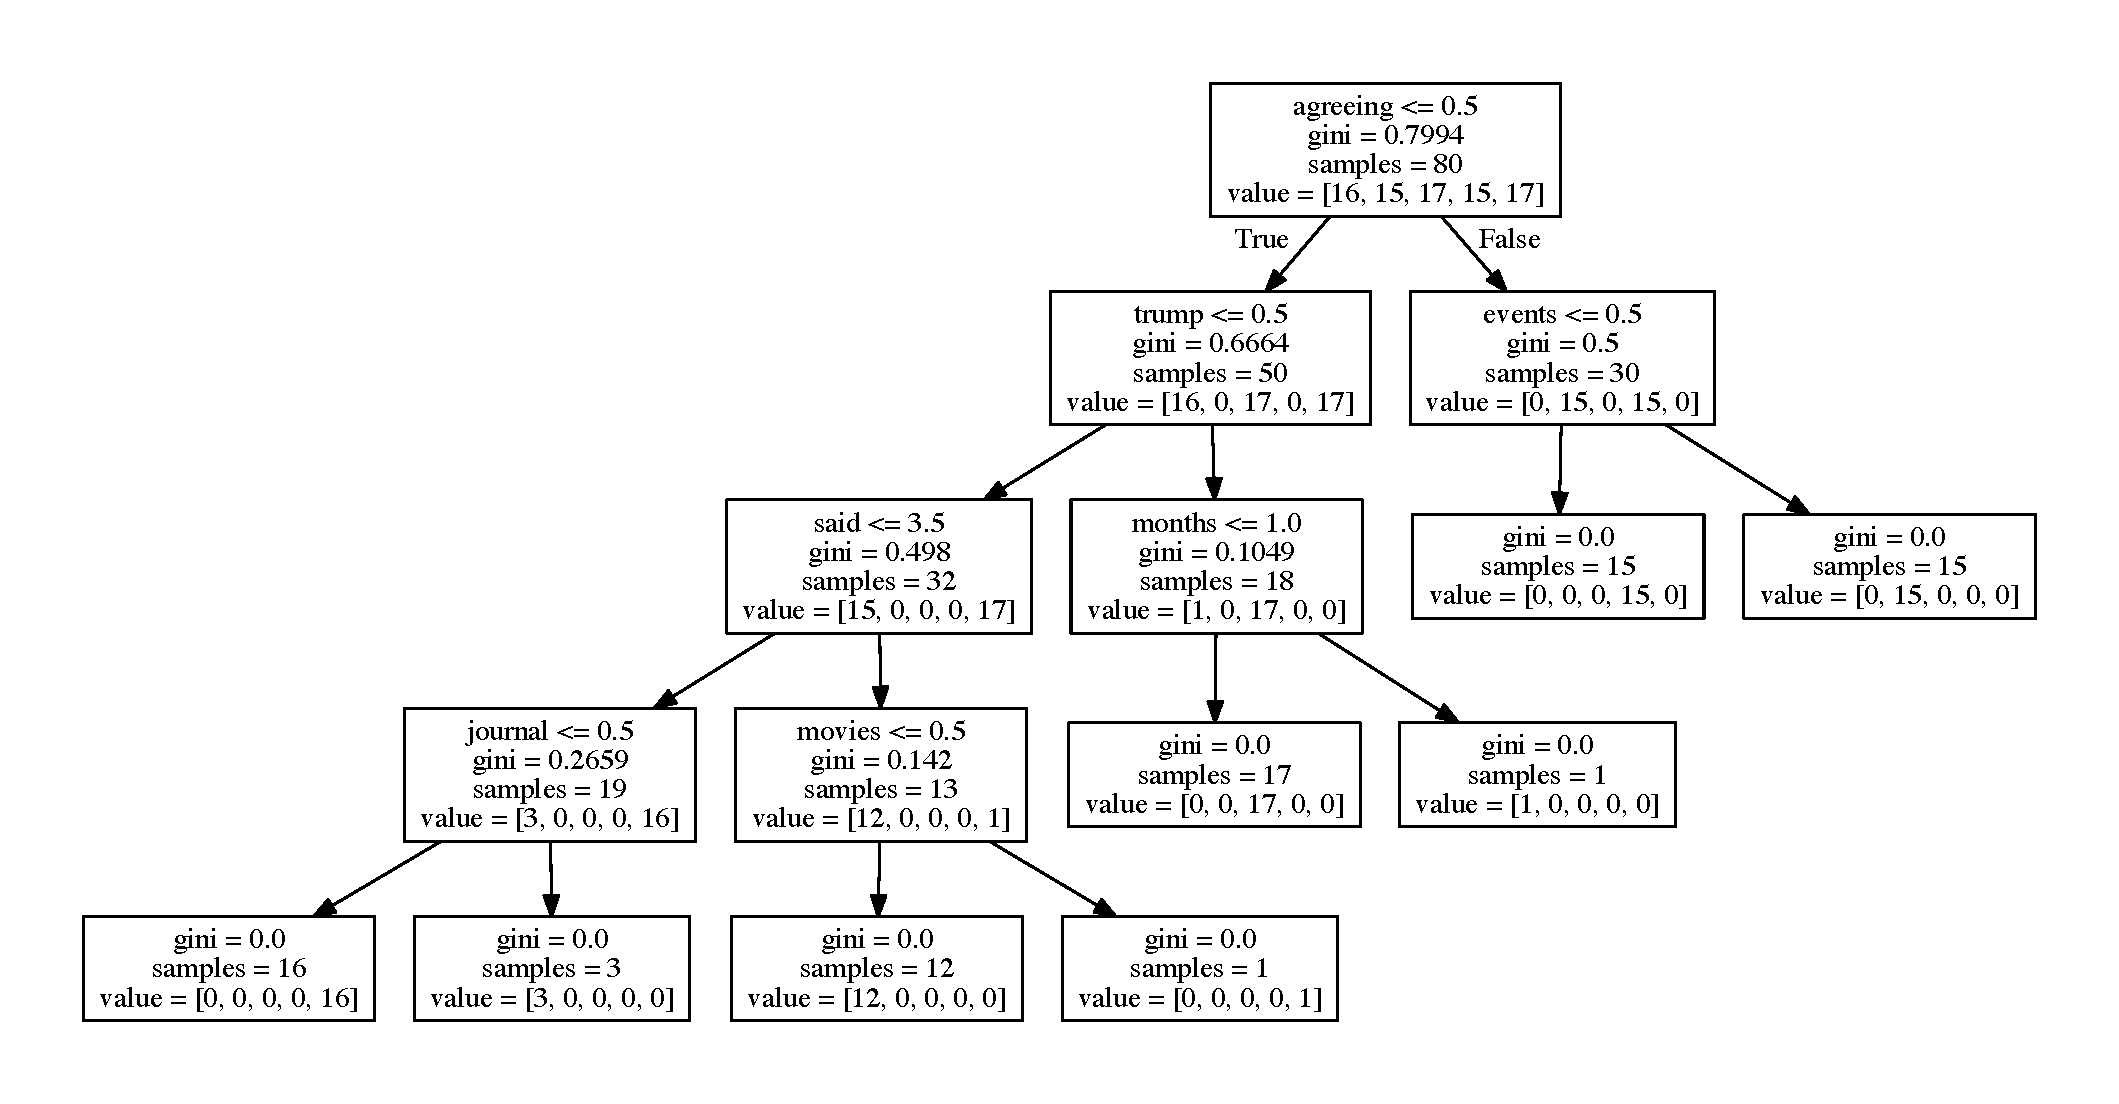
\includegraphics[width=\linewidth]{../1.pdf}
				\caption{Decision Tree, First Fold, Non-Reduced}
				\label{fig:DT1}
			\end{figure}
			\begin{figure}
				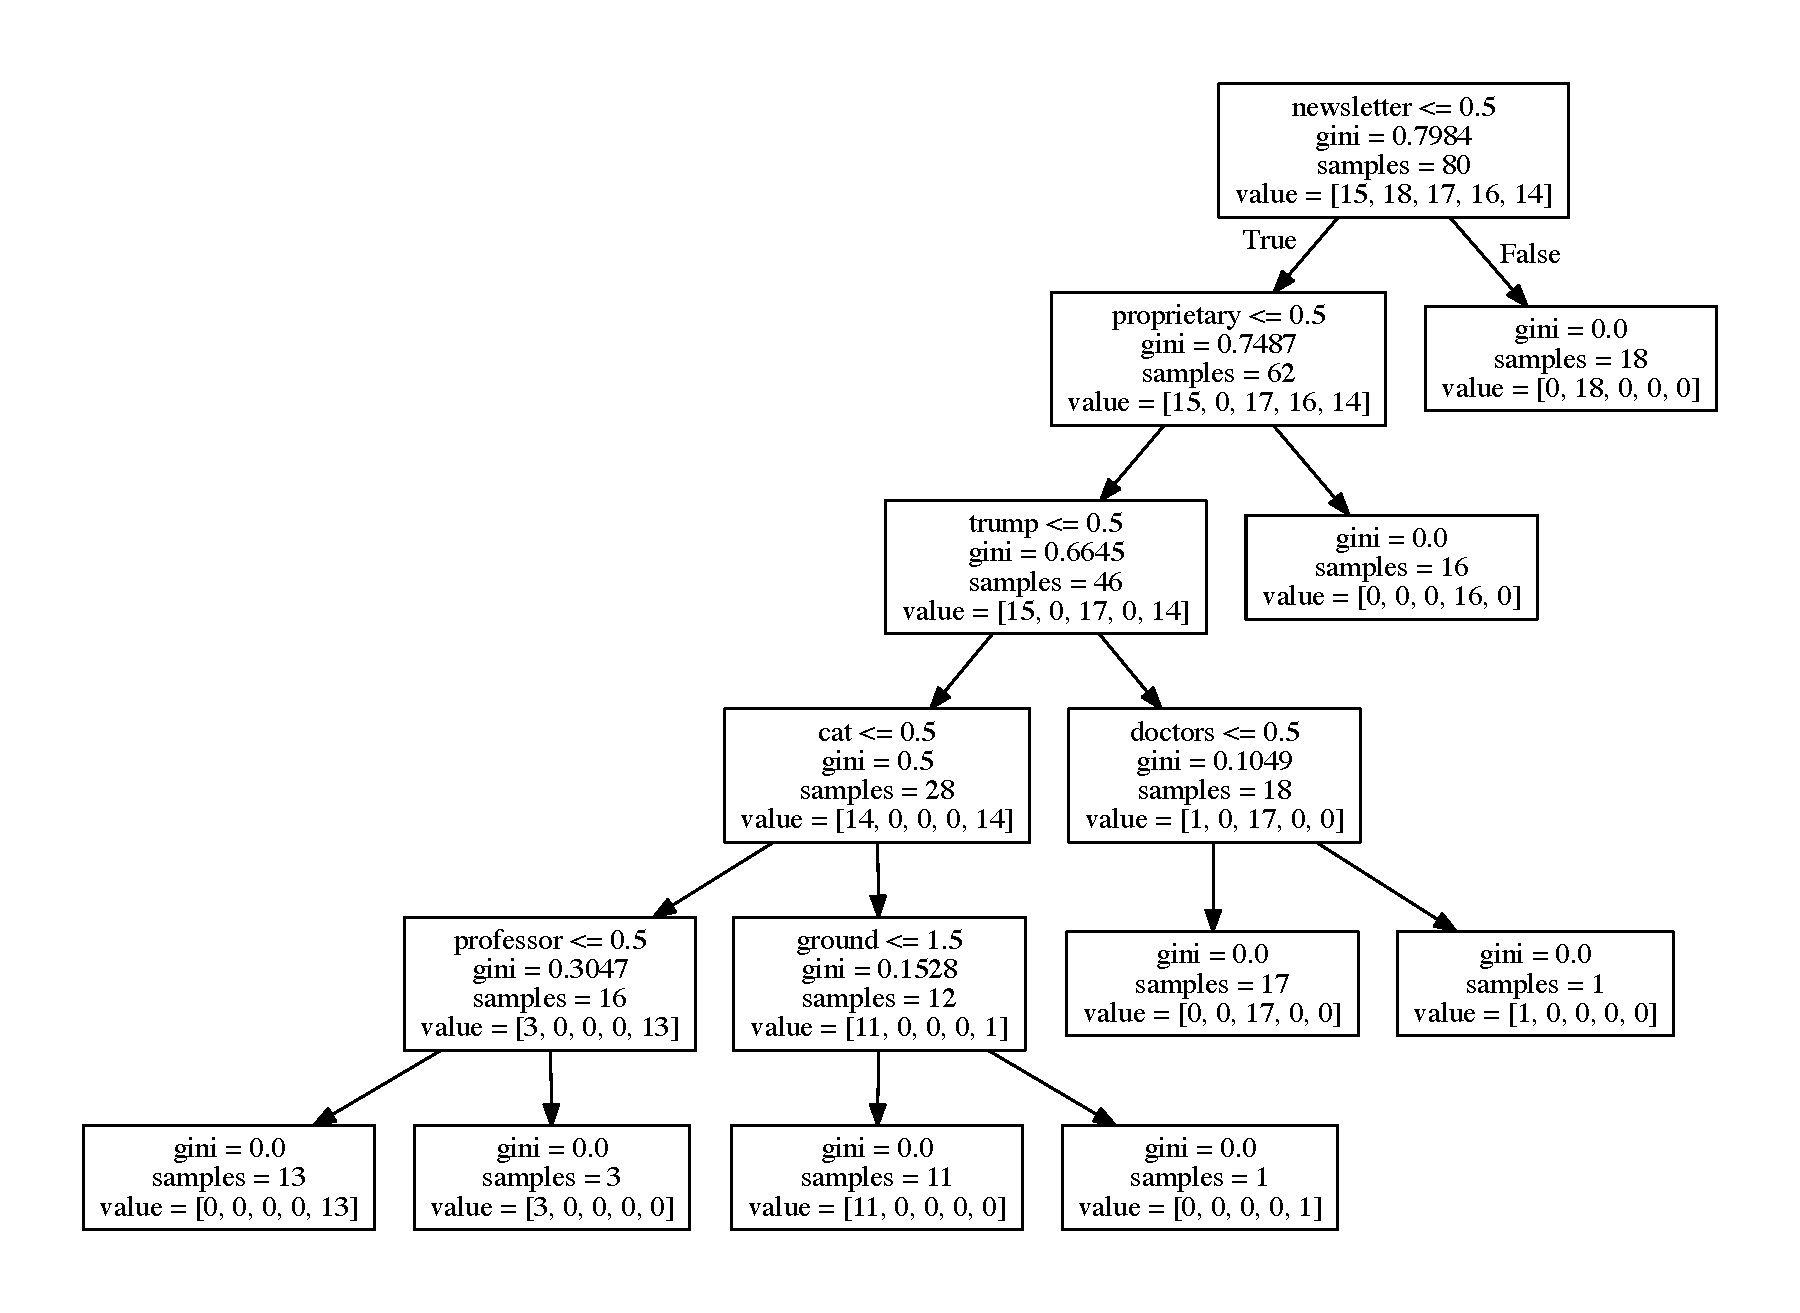
\includegraphics[width=\linewidth]{../2.pdf}
				\caption{Decision Tree, Second Fold, Non-Reduced}
				\label{fig:DT2}
			\end{figure}
			\begin{figure}
				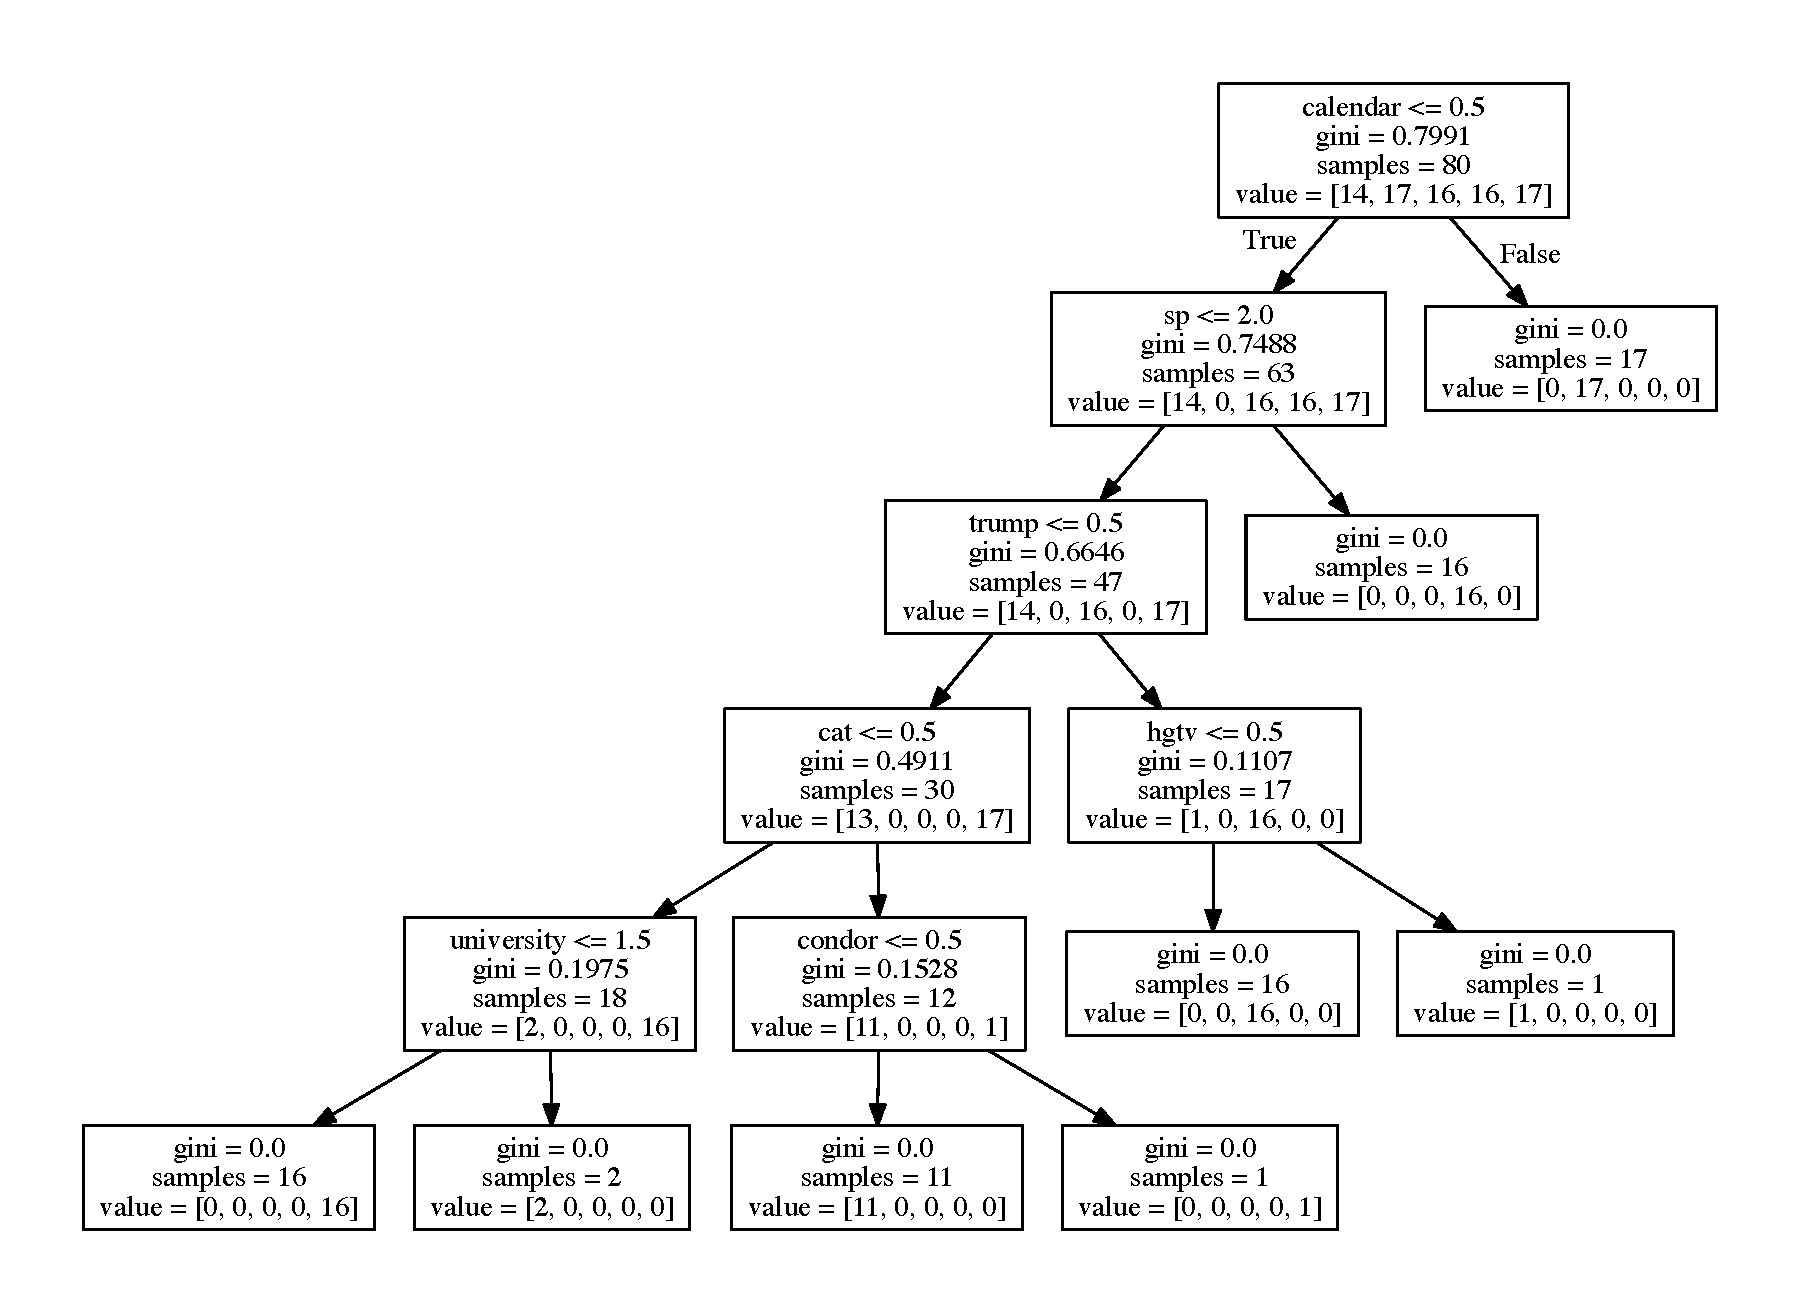
\includegraphics[width=\linewidth]{../3.pdf}
				\caption{Decision Tree, Third Fold, Non-Reduced}
				\label{fig:DT3}
			\end{figure}
			\begin{figure}
				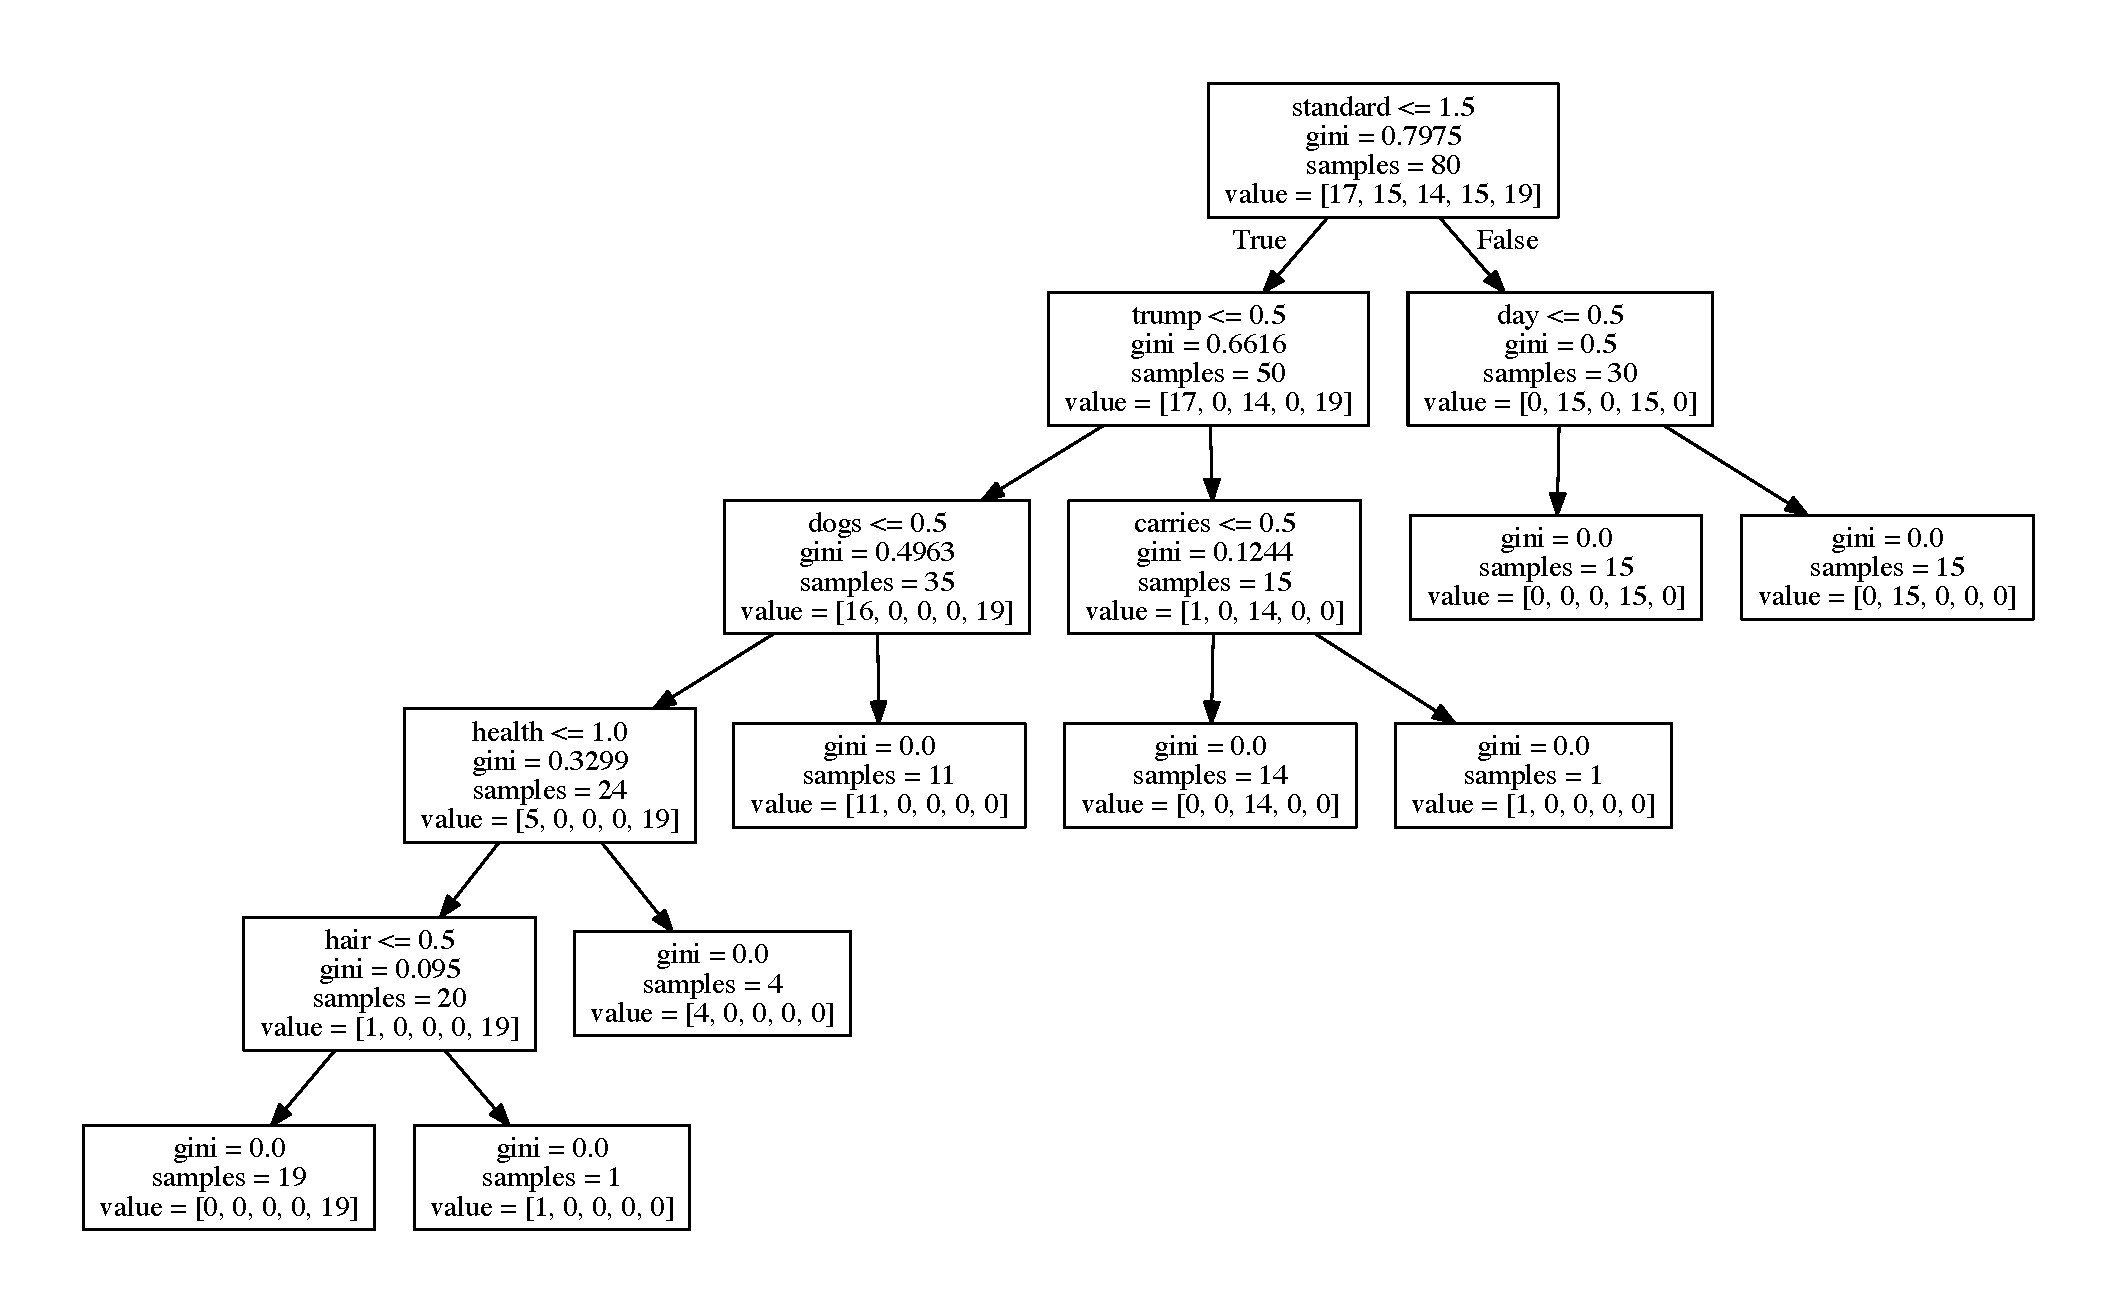
\includegraphics[width=\linewidth]{../4.pdf}
				\caption{Decision Tree, Fourth Fold, Non-Reduced}
				\label{fig:DT4}
			\end{figure}
			\begin{figure}
				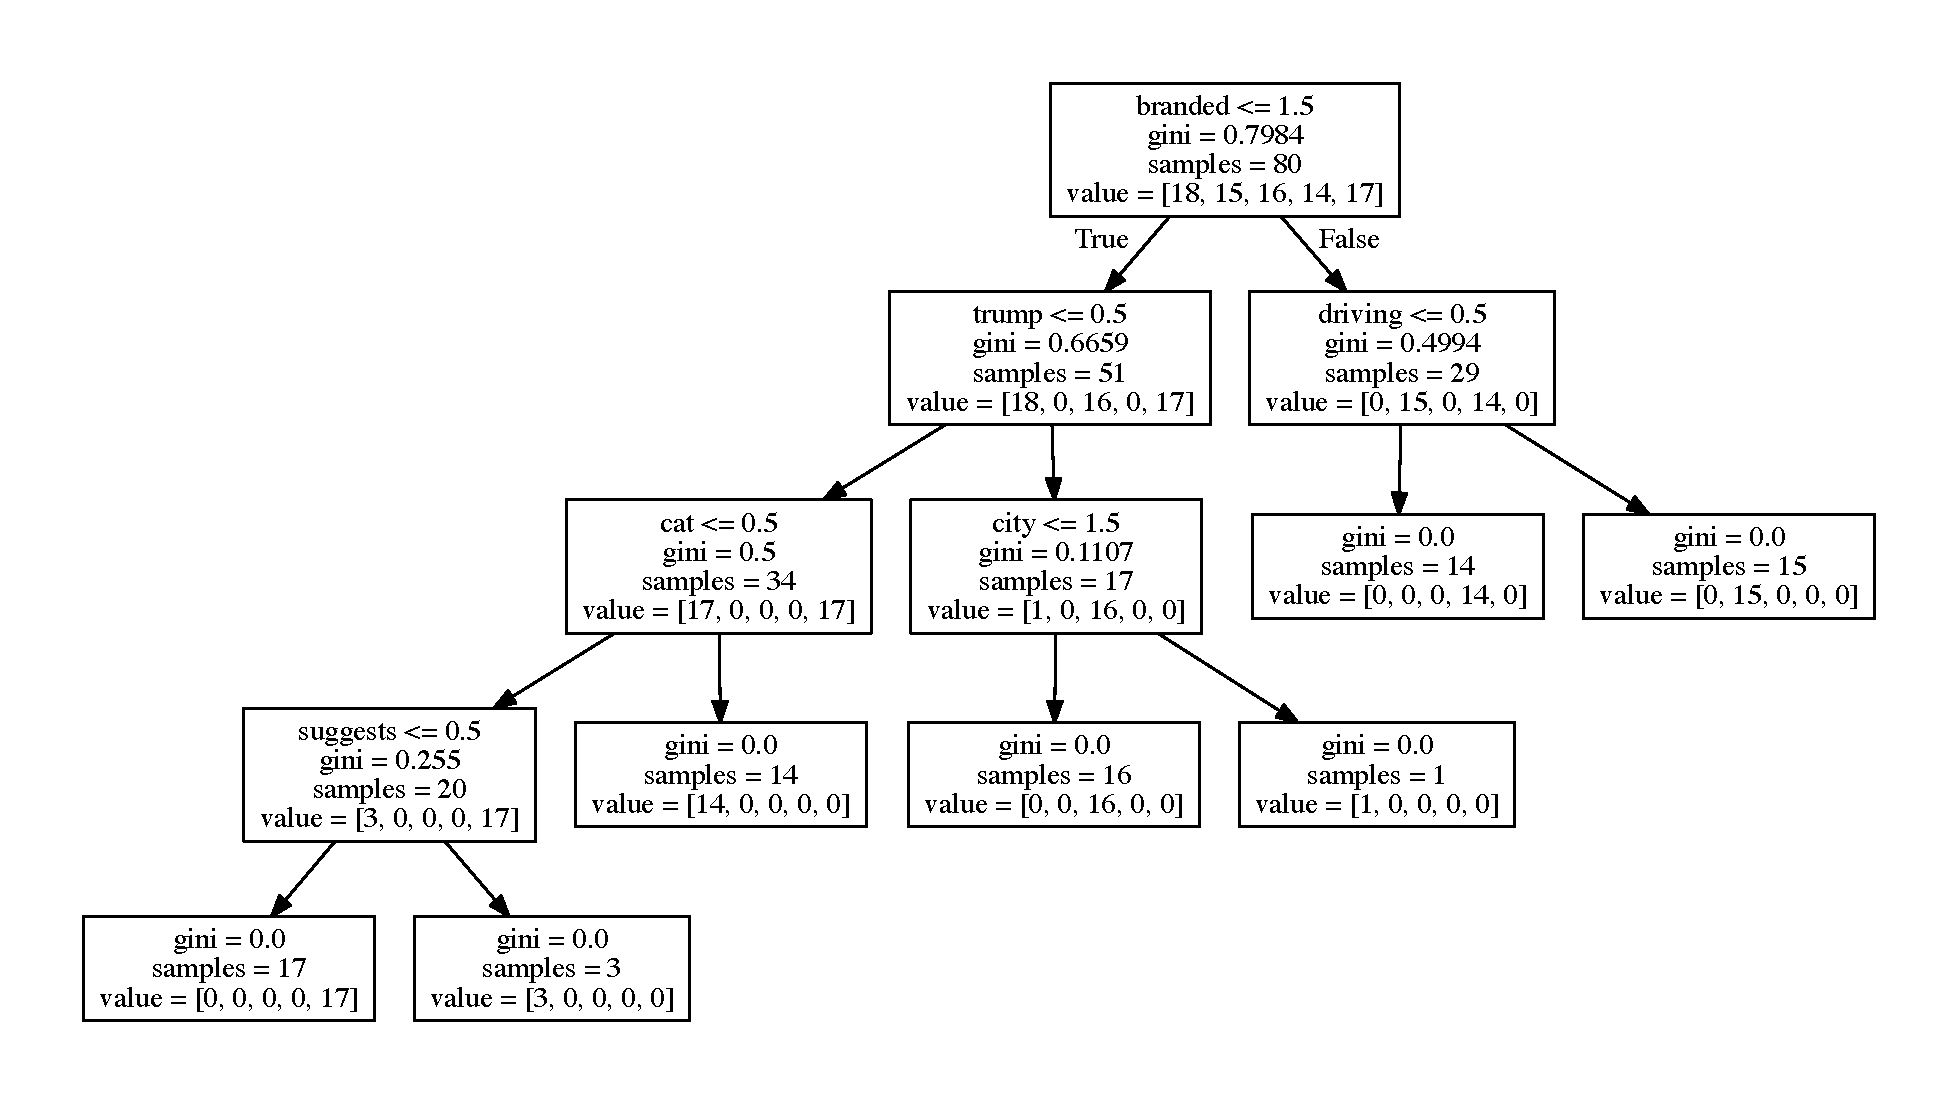
\includegraphics[width=\linewidth]{../5.pdf}
				\caption{Decision Tree, Fifth Fold, Non-Reduced}
				\label{fig:DT5}
			\end{figure}

			\paragraph{}
		 	Decision tree works by finding relationships between attributes of a category vs attributes in other categories. Every non-leaf node has a test. If the test returns true, it goes down one side, if false, it goes down the other side. Leaf nodes represent the category to place that item in. An example is in figure \ref{fig:DT1}. This figure shows the first fold for a 5-fold test.

			\paragraph{}
			As can be seen by figure \ref{fig:DT1}, the root node it \textit{agreeing}. If \textit{agreeing} occurs less than once in the article, then it will go down the left sub-tree. This comparison will continue until a leaf is reached, at which point we will be able to classify the article. Figures \ref{fig:DT2}, \ref{fig:DT3}, \ref{fig:DT4}, and \ref{fig:DT5} show the decision tree for the remainder of the folds. Table \ref{table:DT} shows the accuracy and F-measure of the decision tree.

	\section{Feature Reduction}
		\paragraph{}
		After the data set was ran normally, feature reduction was imposed. Feature reduction finds attributes with low variance and removes them. A variance threshold of 80\% was used in the feature reduction test case. To run feature reduction, the program \textbf{kNN.py} must be ran with the flag \textbf{-r}. The purpose of feature reduction is to reduce the dimension of the data. The reduction of dimensions can have multiple effects. For one, it requires a shorter training time. Another reason is to simplify the model. Third is to avoid the curse of dimensionality. Finally, possibly the most important, is to reduce overfitting. Overfitting is the act of making one's model to precise with the training data. This can cause the model to not perform well under other circumstances, such as with a testing set. After applying feature reduction to the 100 CNN articles, the number of attributes went from 11890 to 1239, a nine and a half time reduction in attributes.

		\begin{figure}
			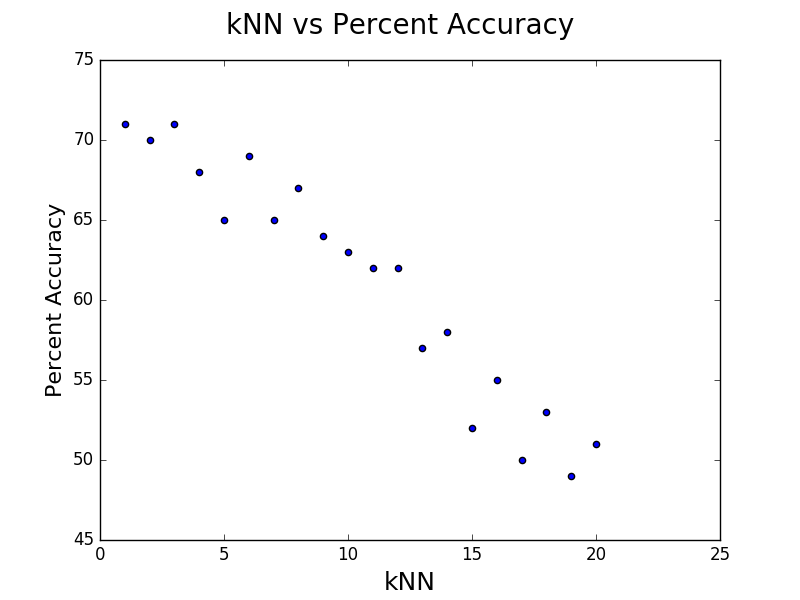
\includegraphics[width=\linewidth]{../kNNvsNum_Reduced.png}
			\caption{kNN vs Percent Accuracy, Feature Reduction}
			\label{fig:kNNvsNum_reduced}
		\end{figure}

		\begin{table}[h!]
			\centering
			\resizebox{\textwidth}{!}{
			\begin{tabular}{ |c|c|c| } 
				 \hline
				 Nodes 	& Accuracy	& F-measure \\ 
				 \hline
				 1 		& 72.0\% 	& [0.67230769230769227, 0.66249999999999998, 0.89612942612942614, 0.69999999999999996, 0.51089743589743586] \\ 
				 2 		& 74.0\% 	& [0.73333333333333328, 0.5714285714285714, 0.89612942612942614, 0.74523809523809526, 0.50936507936507947] \\ 
				 3 		& 67.0\% 	& [0.63119658119658117, 0.52788461538461529, 0.89612942612942614, 0.49423076923076925, 0.53041666666666676] \\ 
				 4 		& 69.0\% 	& [0.68333333333333335, 0.56634615384615383, 0.83335164835164832, 0.55126540126540124, 0.53347222222222224] \\ 
				 5 		& 63.0\% 	& [0.57873015873015876, 0.54166666666666663, 0.73168498168498164, 0.49423076923076925, 0.52083333333333326] \\ 
				 6 		& 68.0\% 	& [0.63958333333333328, 0.55673076923076914, 0.78880619380619388, 0.60256410256410253, 0.57847222222222228] \\ 
				 7 		& 64.0\% 	& [0.63958333333333328, 0.55673076923076914, 0.73168498168498164, 0.46298701298701295, 0.53041666666666676] \\ 
				 8 		& 68.0\% 	& [0.63958333333333328, 0.6067307692307693, 0.73168498168498164, 0.55126540126540124, 0.62624999999999997] \\ 
				 9 		& 61.0\% 	& [0.57705882352941174, 0.6067307692307693, 0.64642857142857135, 0.33659340659340659, 0.52428104575163403] \\ 
				 10		& 63.0\% 	& [0.58958333333333335, 0.6067307692307693, 0.64642857142857135, 0.42487179487179488, 0.57205882352941173] \\ 
				 11		& 61.0\% 	& [0.63958333333333328, 0.6067307692307693, 0.64642857142857135, 0.33659340659340659, 0.47622549019607846] \\ 
				 12		& 60.0\% 	& [0.58958333333333335, 0.6067307692307693, 0.64642857142857135, 0.33659340659340659, 0.47622549019607846] \\ 
				 13		& 54.0\% 	& [0.4620588235294118, 0.44333333333333336, 0.64642857142857135, 0.33659340659340659, 0.39305555555555549] \\ 
				 14		& 55.0\% 	& [0.4620588235294118, 0.50714285714285712, 0.64642857142857135, 0.33659340659340659, 0.39305555555555549] \\ 
				 15		& 51.0\% 	& [0.4620588235294118, 0.44333333333333336, 0.5180769230769231, 0.33659340659340659, 0.33888888888888891] \\ 
				 16		& 51.0\% 	& [0.4620588235294118, 0.44333333333333336, 0.5180769230769231, 0.33659340659340659, 0.33991596638655464] \\ 
				 17		& 51.0\% 	& [0.4620588235294118, 0.44333333333333336, 0.5180769230769231, 0.33659340659340659, 0.34355158730158736] \\ 
				 18		& 49.0\% 	& [0.4620588235294118, 0.44333333333333336, 0.5180769230769231, 0.33659340659340659, 0.28636363636363638] \\ 
				 19		& 46.0\% 	& [0.3725133689839572, 0.38916666666666666, 0.5180769230769231, 0.33659340659340659, 0.27781385281385279] \\ 
				 20		& 48.0\% 	& [0.4620588235294118, 0.38916666666666666, 0.5180769230769231, 0.33659340659340659, 0.34642857142857142] \\ 	 
				 \hline
			\end{tabular}}
			\caption{Accuracy and F-measure of kNN from k=1 to 20 with Feature Reduction}
			\label{table:kNN_reduced}
		\end{table}


		\begin{table}[h!]
			\centering
			\resizebox{\textwidth}{!}{
			\begin{tabular}{ |c|c| } 
				 \hline
				 Accuracy 	& F-measure \\ 
				 \hline
				 92.0\% 	& [0.89333333333333331, 0.9494949494949495, 0.9485714285714284, 0.95079365079365064, 0.8504870129870129] 	\\ 
				 \hline
			\end{tabular}}
			\caption{Accuracy and F-measure of the Decision Tree with Feature Reduction}
			\label{table:DT_reduced}
		\end{table}

		\begin{figure}
			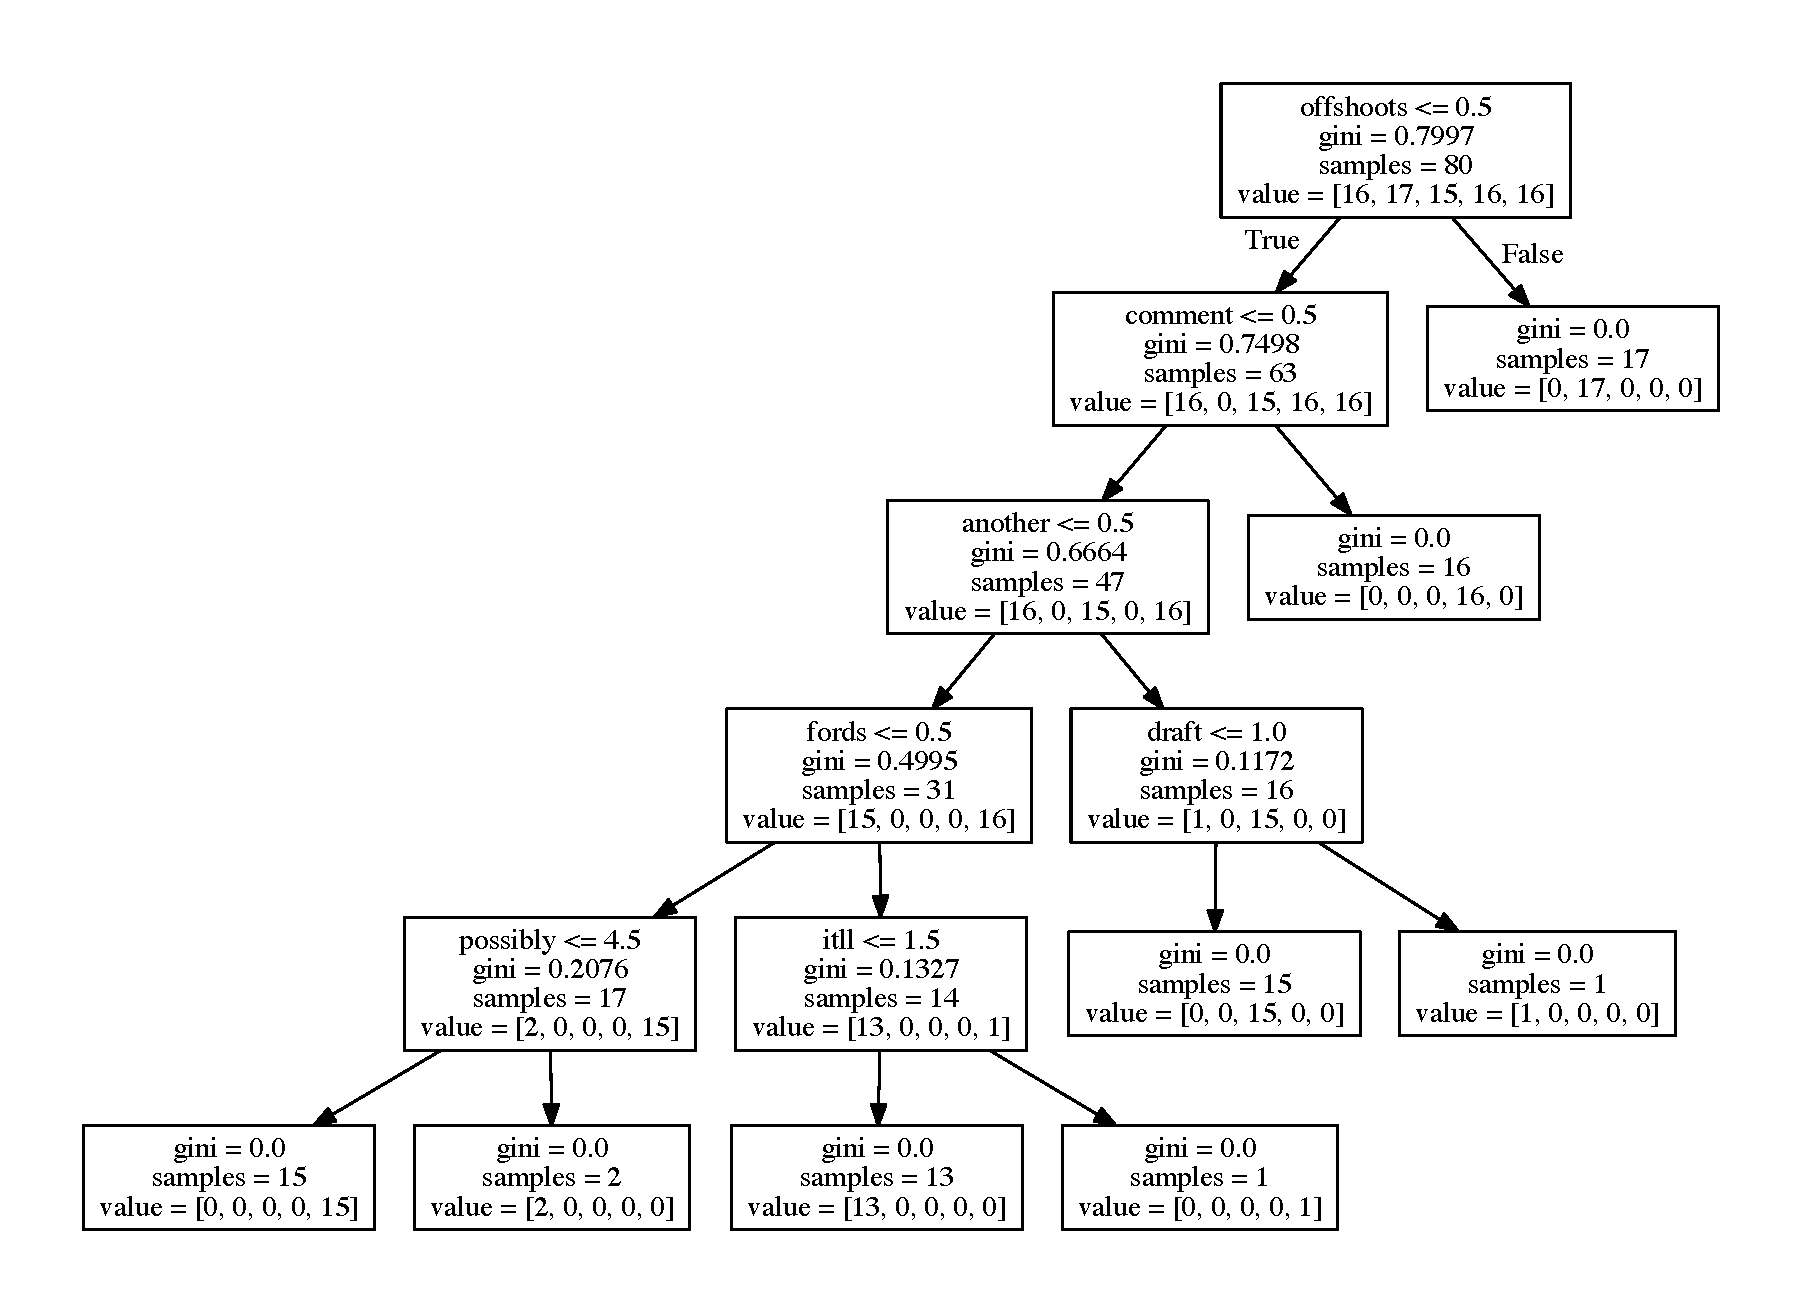
\includegraphics[width=\linewidth]{../1_reduced.pdf}
			\caption{Decision Tree, First Fold, Feature Reduction}
			\label{fig:DT1_reduced}
		\end{figure}
		\begin{figure}
			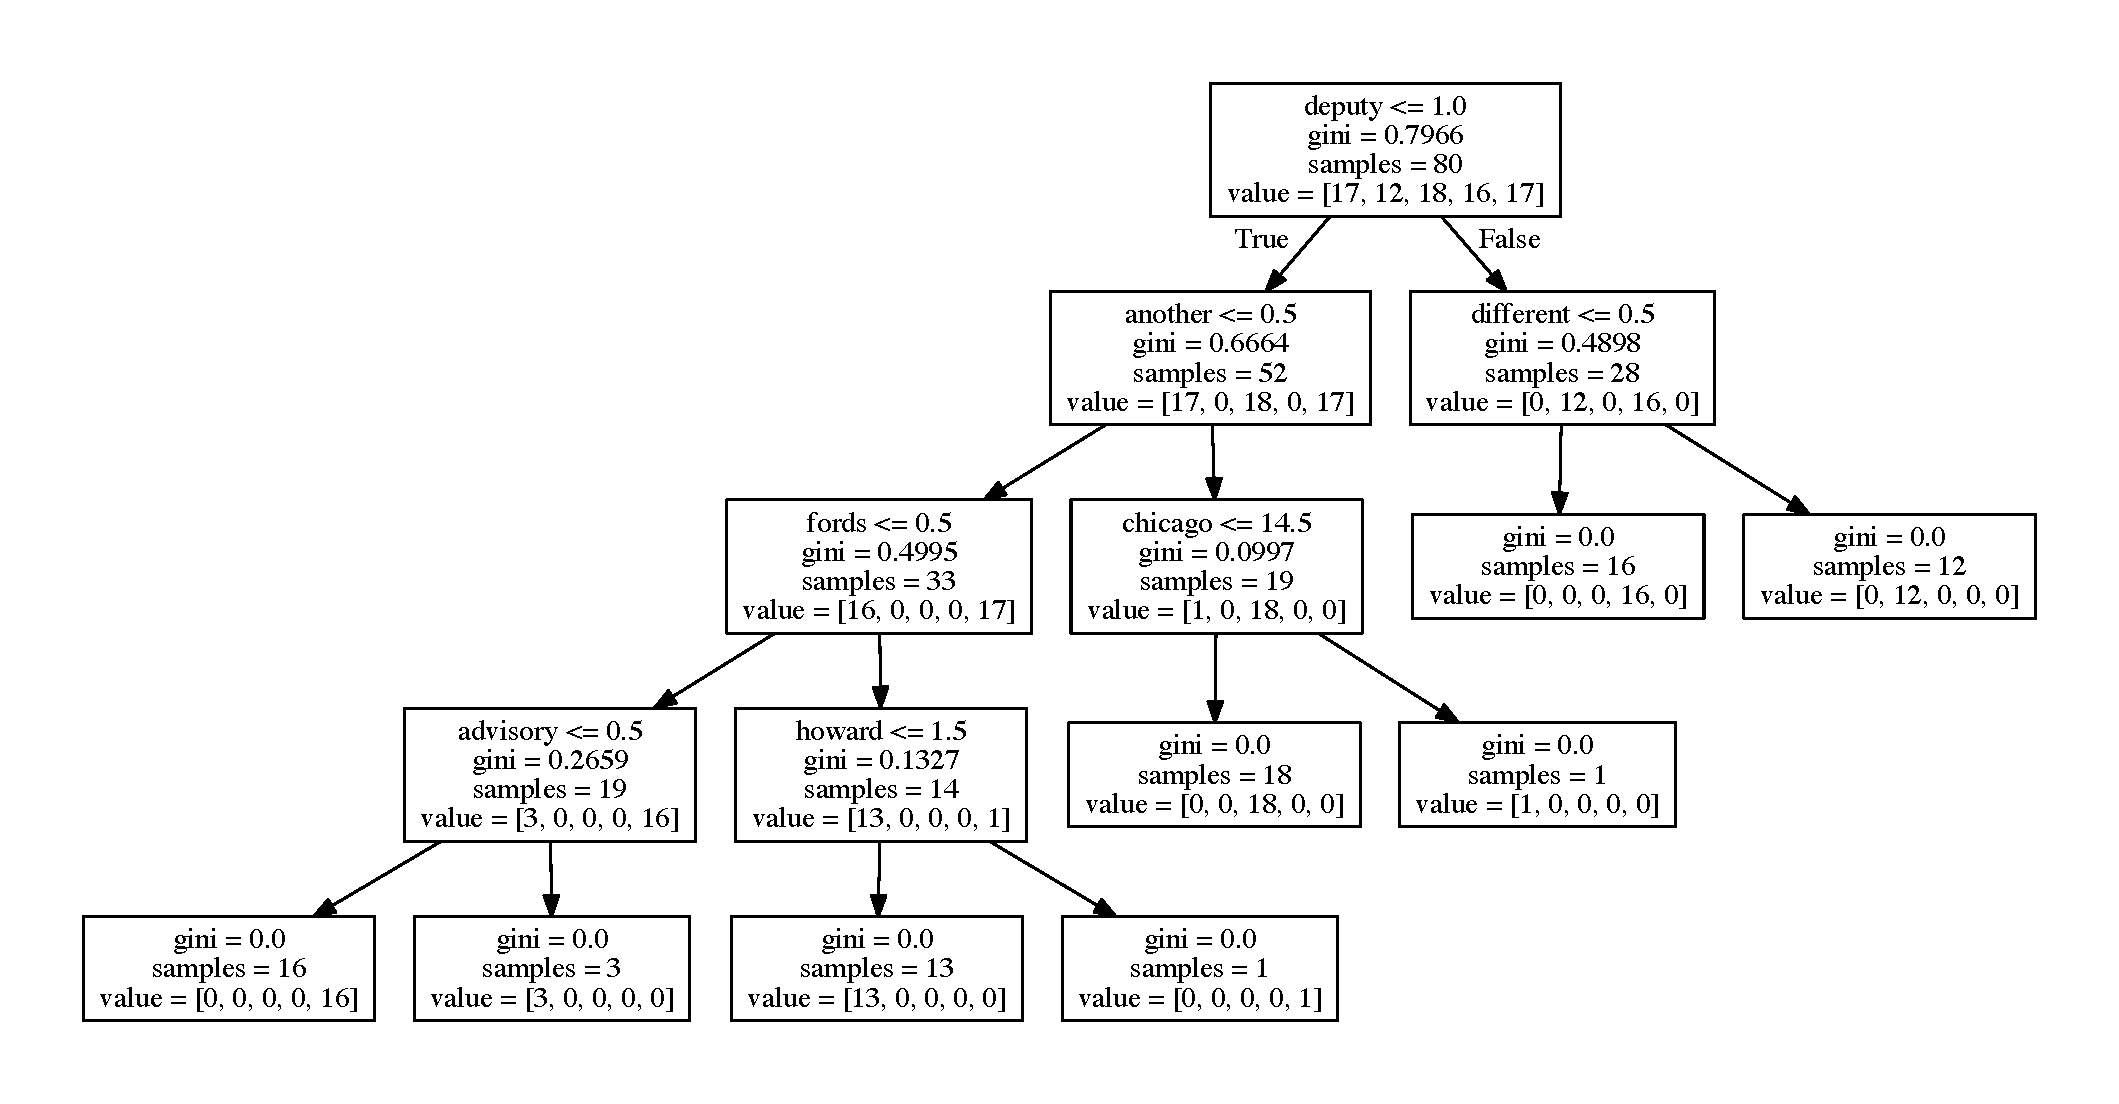
\includegraphics[width=\linewidth]{../2_reduced.pdf}
			\caption{Decision Tree, Second Fold, Feature Reduction}
			\label{fig:DT2_reduced}
		\end{figure}
		\begin{figure}
			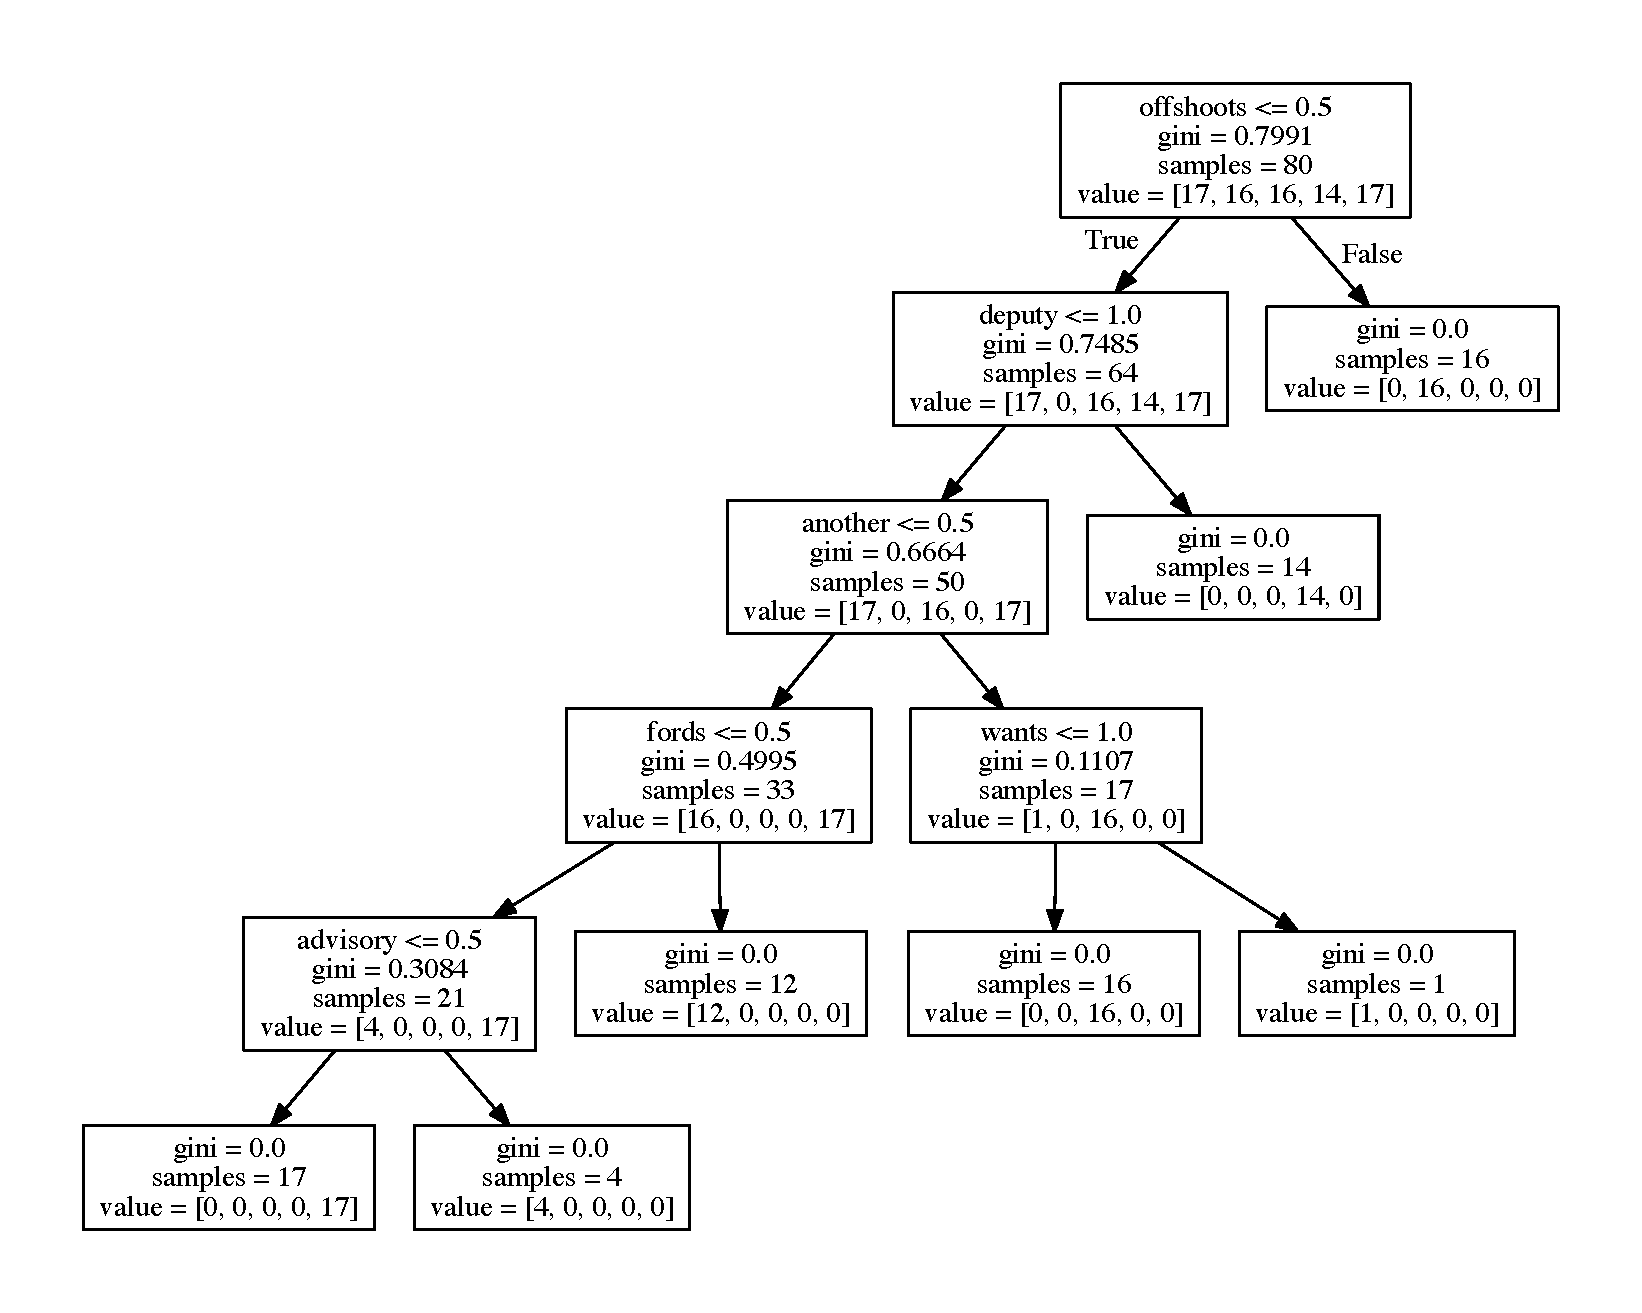
\includegraphics[width=\linewidth]{../3_reduced.pdf}
			\caption{Decision Tree, Third Fold, Feature Reduction}
			\label{fig:DT3_reduced}
		\end{figure}
		\begin{figure}
			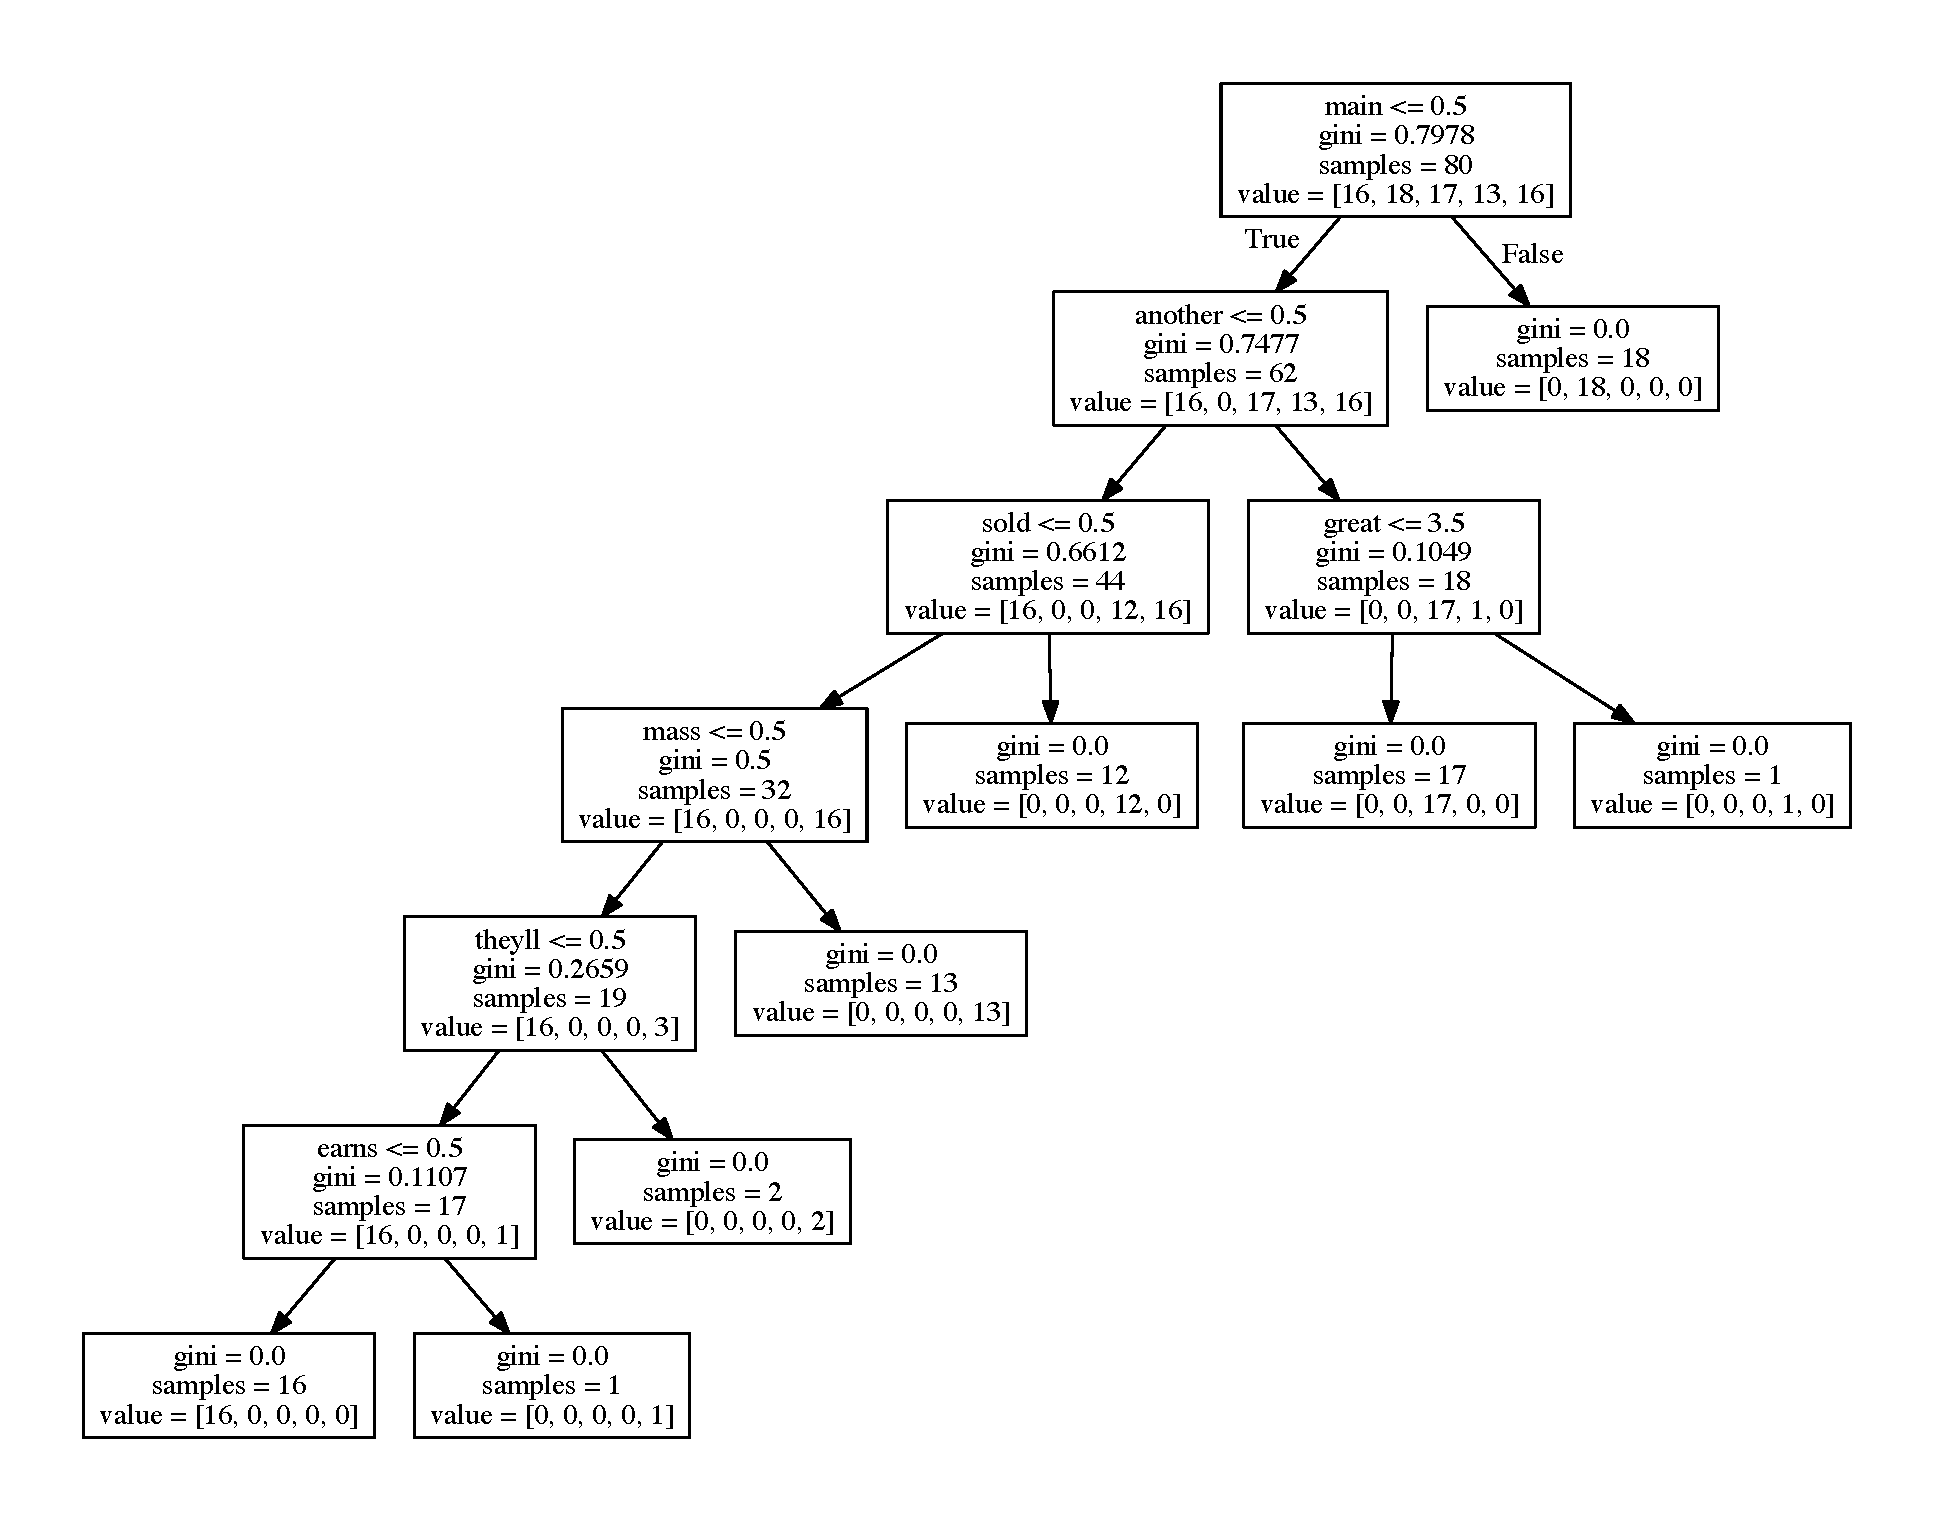
\includegraphics[width=\linewidth]{../4_reduced.pdf}
			\caption{Decision Tree, Fourth Fold, Feature Reduction}
			\label{fig:DT4_reduced}
		\end{figure}
		\begin{figure}
			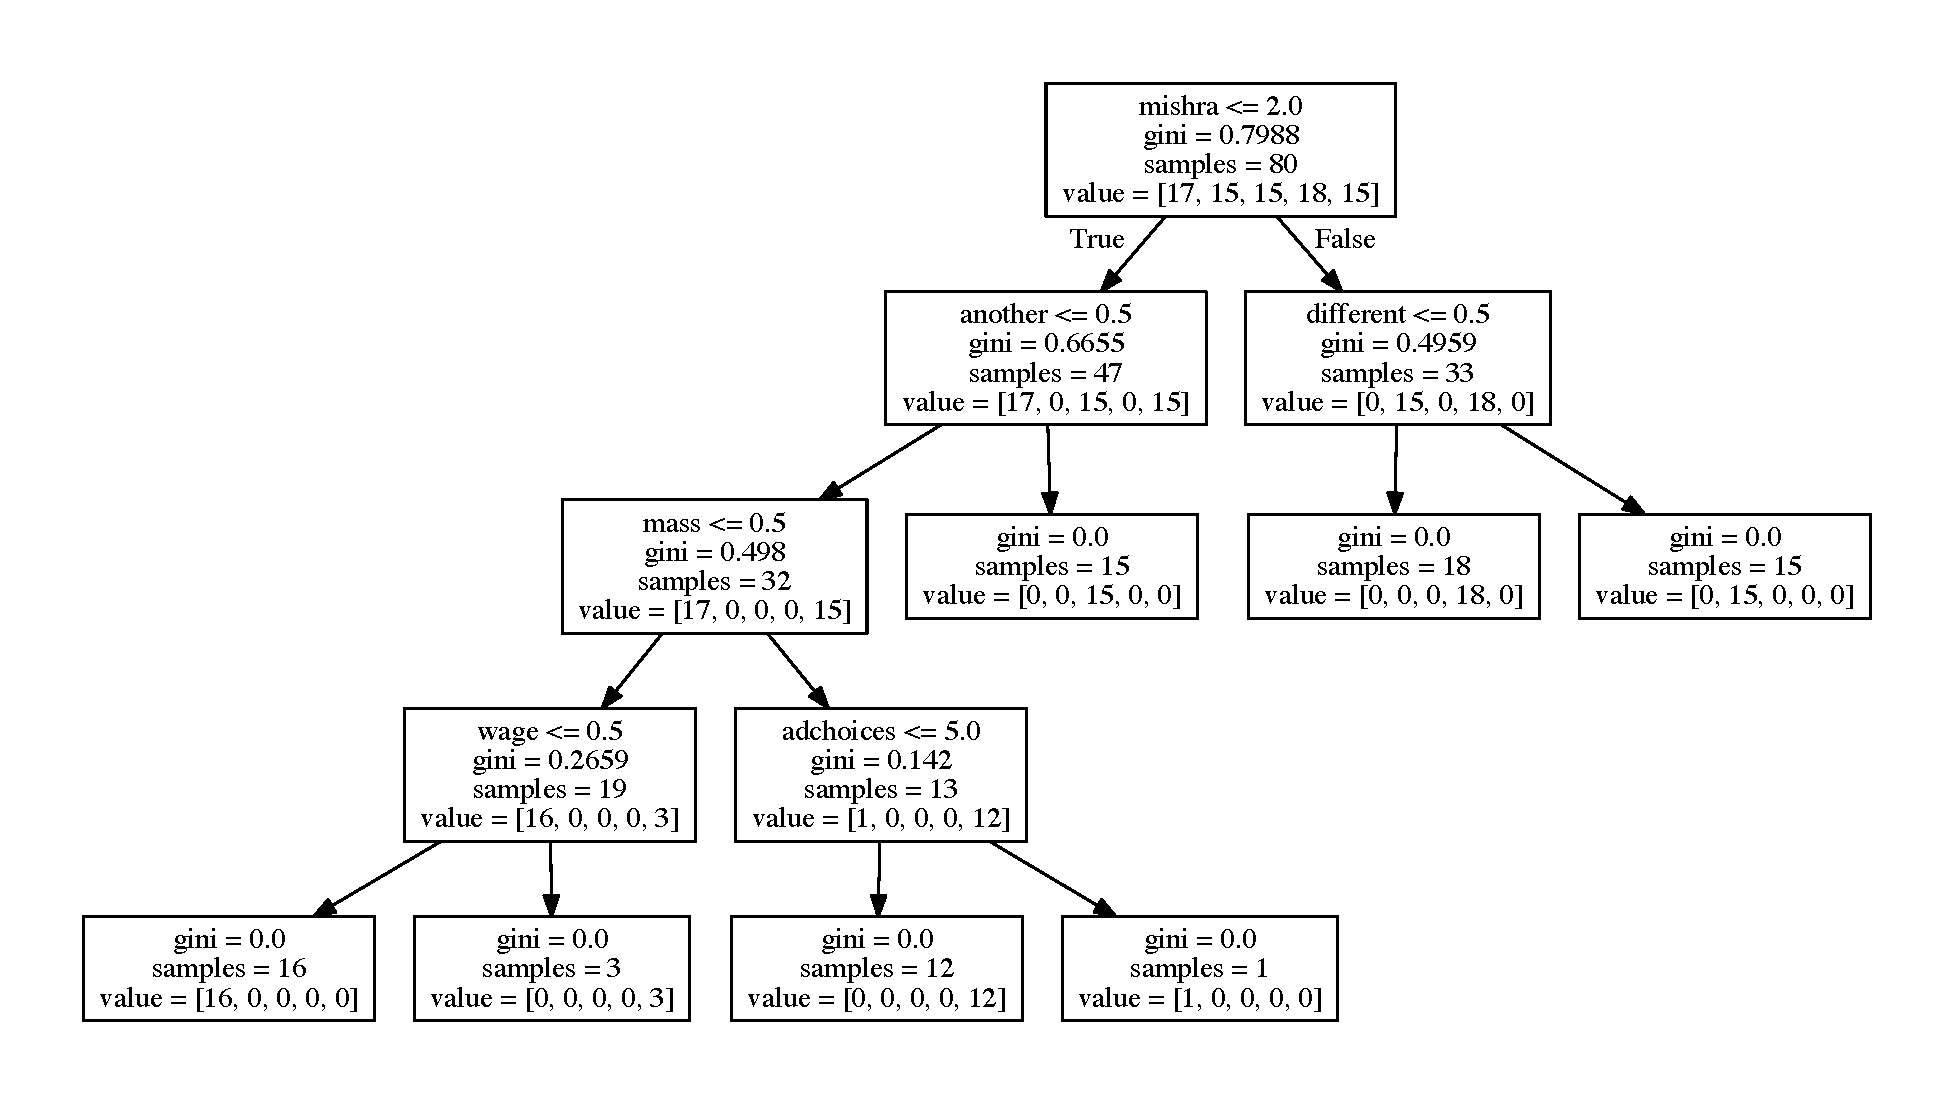
\includegraphics[width=\linewidth]{../5_reduced.pdf}
			\caption{Decision Tree, Fifth Fold, Feature Reduction}
			\label{fig:DT5_reduced}
		\end{figure}

		\paragraph{}
		Tables \ref{table:kNN_reduced} and \ref{table:DT_reduced} shows the kNN and decision tree results, respectively. Figure \ref{fig:kNNvsNum_reduced} shows the kNN accuracy for different values of k. Figures \ref{fig:DT1_reduced}, \ref{fig:DT2_reduced}, \ref{fig:DT3_reduced}, \ref{fig:DT4_reduced}, and \ref{fig:DT5_reduced} shows the decision tree for each fold.

	\section{Conclusion}
		\paragraph{kNN vs Decision Trees}
		As the above tests have shown, decision trees outperform kNN classifiers by a fair margin. This test was ran multiple times on this data set, and decision trees won over kNN classifiers every time. The only change when re-running the program is what data is in each fold. 

		\paragraph{k in kNN}
		With both the feature reduced and non-feature reduced kNN classifiers, a low k proved to be superior. A k of 1 worked best for the non-feature reduced kNN classifier and a k of 2 worked best for the feature reduced case. This is of a small difference. As k increased, the accuracy and F-measure decreased in both cases.

		\paragraph{Feature Reduction vs None}
		Feature reduction was superior over no feature reduction in both the kNN and decision tree case. The margin as to which it was better was slim in both cases. The run time difference between the two was severe however. When generating the data in this report, the normal case ran in 36 seconds. The feature reduction case ran in just under 5 seconds. That is an over seven fold time gain. The feature reduction itself does cause some overhead, but in this case, enough features were removed to make the overhead well worth it.


\end{document}	 








